\subsection{Improper Curves}

\begin{definition}
  An \emph{A-graph} (AD-HOC TERM, THINK OF A BETTER NAME)
is a graph $G$ together with a Jordan curve/arc $C$ that intersects
every edge of $C$ in exactly one point, possibly an endpoint,
and where every vertex on $C$ has at least one incident edge on each side.
\end{definition}

They have the following properties:

\begin{enumerate}
\item Every face, including the outer face, is a quadrilateral or a
  triangle.
\item Every $v$ vertex on $C$ is incident to precisely two triangles,
  one 
above $v$ and one below $v$. (This holds also when $v$ is a boundary
vertex; in this case, one of the triangles is the other face.)
\item Every triangle face contains one vertex on $C$, one vertex in
  $L$ and one vertex in $R$.
\item Every vertex is incident to at least two edges.
\item Every vertex on $C$ is incident to at least three edges.
EXCEPTION: If $v$ is on the outer face, it can have degree 2.
WE MUST EXCLUDE THE DEGREE-2 CASE SOMEWHERE. IT IS TRIVIAL TO HANDLE.
I DON'T KNOW WHERE THE PROPER PLACE FOR HANDLING IT.
\end{enumerate}

\begin{thm}\thmlabel{a-graph}
(Generalization of \thmref{quad})

   Let
   \begin{compactenum}
     \item  $G$ be an A-graph;
     \item  $C:[0,1]\to\R^2$ be an admissible Jordan curve for $T$;
     \item $r_1,\ldots,r_k \subseteq E(V)\cup E(G)$ be the sequence of vertices and open edges
           of $T$ that are intersected by $C$, in the order
           that they are intersected by $C$;
     \item $y_1<\cdots<y_k$ be any sequence of numbers; and
     \item .... [$\Delta$ be a triangle that is compatible with 
           $r_1,\ldots,r_m$ and $y_1,\ldots,y_m$.]
  \end{compactenum}
$G$ has a
   \Fary\ embedding in which the outer face $f$ [ is $\Delta$ ]
   and, for each $i\in\{1,\ldots,k\}$, 
   \begin{compactenum}
       \item if $r_i$ is a vertex, then $r_i$ is drawn on the y-axis, with y-coordinate $y_i$;
%       \item if $r_i$ is an edge contained in $C$, then $r_i$ is drawn so that
%         it is contained in the y-axis; or
       \item If $r_i$ is an edge whose intersection with $C$ is a
         single point interior to $r_i$, 
         the intersection of $r_i$ with the
         y-axis has y-coordinate
         $y_i$.
   \end{compactenum}
\end{thm}

\begin{proof}
  We will describe the straight-line embedding by assigning a slope $s_e$
to every edge $e\in E$.
Since there can be no vertical edges, the slopes are well-defined.
We have $m=|E|$ slope variables.

Since every edge goes through a point on the y-axis with known
coordinate, the slope fixes the line through the edge.
 Since
every vertex not on $C$ is incident to at least two edges that go
through
distinct points on the y-axis, location of such a vertex is fixed.

A necessary condition for the slopes is that the lines of edges that
go through a common vertex should be concurrent:
We can extend the function $y$ to all edges, independently of how they
intersect $C$. If $e$ intersects $C$ at an endpoint, we let $y_e$ be
the
given $y$-coordinate of that endpoint. THINK ABOUT A BETTER NOTATION!
%
Let $v$ be a vertex $v$ not on $C$, and let $e_i, e_j, e_k$ be three
edges incident to $v$.
The fact that the three supporting lines of $e_i$, $e_j$, and $e_k$ 
meet at a common point (the location of $v$) is expressed
the following \emph{concurrency constraint} 
in terms of the slopes $s_i,s_j,s_k$:
\begin{equation}\eqlabel{slope0} 
\left|
  \begin{matrix}
    1&1&1\\
s_i&s_j&s_k\\
y_i&y_j&y_k
  \end{matrix}
\right|=
   ({y_j-y_k}) s_i + ({y_k-y_i}) s_j 
          + ({y_i-y_j})s_k  = 0
\end{equation}
Since $y_1,\ldots,y_m$ are given, this is a linear equation
in $s_1,\ldots,s_m$.
Writing this equation for all triplets of edges incident to a common
vertex will include many redundant equations.
If $d_v$ edges meet in a vertex~$v$, 
 It suffices to take $d_v-2$ equations: We choose two fixed
incident edges $e_i$ and $e_j$ and run $e_k$ through the remaining
$d-2$ edges, specifying that $e_k$ should go through the common vertex
of $e_i$ and $e_j$.

It will be important to have as many equations as variables;
thus, we add some more equations for the edges that emanate from a
vertex on $C$.
Suppose that edges $a_1,\ldots,a_k$ 
go to the left and edges $b_1,\ldots,b_l$ go to the
right, from bottom to top.
We have $k,l\ge1$ and $k+l\ge 3$.
Let us first look at the slopes on the right side.
We want these slopes to be increasing:
$s_{b_1} < s_{b_2} < \dots  <s_{b_l}$. We stipulate a stronger
condition:
We require that the slopes
$s_{b_2}, \dots, s_{b_{l-1}}$ partition the interval
$[s_{b_1},s_{b_l}]$ in fixed proportions. In other words
\begin{equation}
  \label{eq:proportion}
s_{b_i} = s_1 + \lambda_i(s_{b_{l}}-s_{b_1}),
\end{equation}
for some fixed sequence $0<\lambda_2<\cdots<\lambda_{l-1}<1$.
For example, we might set $\lambda_i := (i-1)/(l-1)$.
This gives $l-2$ equations, for $l\ge 2$. Similarly, we get
$k-2$ equations for the slopes
$s_{a_1}, \dots, s_{a_{k}}$ on the left side, for $k\ge 2$.
In addition, for $k\ge 2$ and $l\ge 2$, we require that the \emph{range} of
slopes
on the two sides are in a fixed proportion
\begin{equation}
  \label{eq:proportion2}
s_{a_1}-s_{a_{k}} = \mu (s_{b_{l}}-s_{b_1}),
\end{equation}
for some fixed value $\mu>0$.

We call the equations
\thetag{\ref{eq:proportion}--\ref{eq:proportion2}} the
\emph{proportionality constraints}.
There are $(k+l)-3$ such equations for the $k+l$ slopes. In
other words, we have three degrees of freedom for the slopes out of a vertex
 \figref{proportional} illustrates these  degrees of freedom:
We can shear the edges on the right side, by adding a constant to all
slopes.
and we can independently shear all edges on the left side.
In addition, we can vertically scale \emph{all} lines jointly (both to
the left and to the right), multiplying all slopes by a constant factor.
If this factor is negative, we would reverse the order of the
slopes. We will later see that other constraints prevent this.


The notations
$\lambda_i$ and 
$\mu$ are here used in a local sense; for a different vertex $v$, we may
choose different constants.
\begin{figure}
     \centering{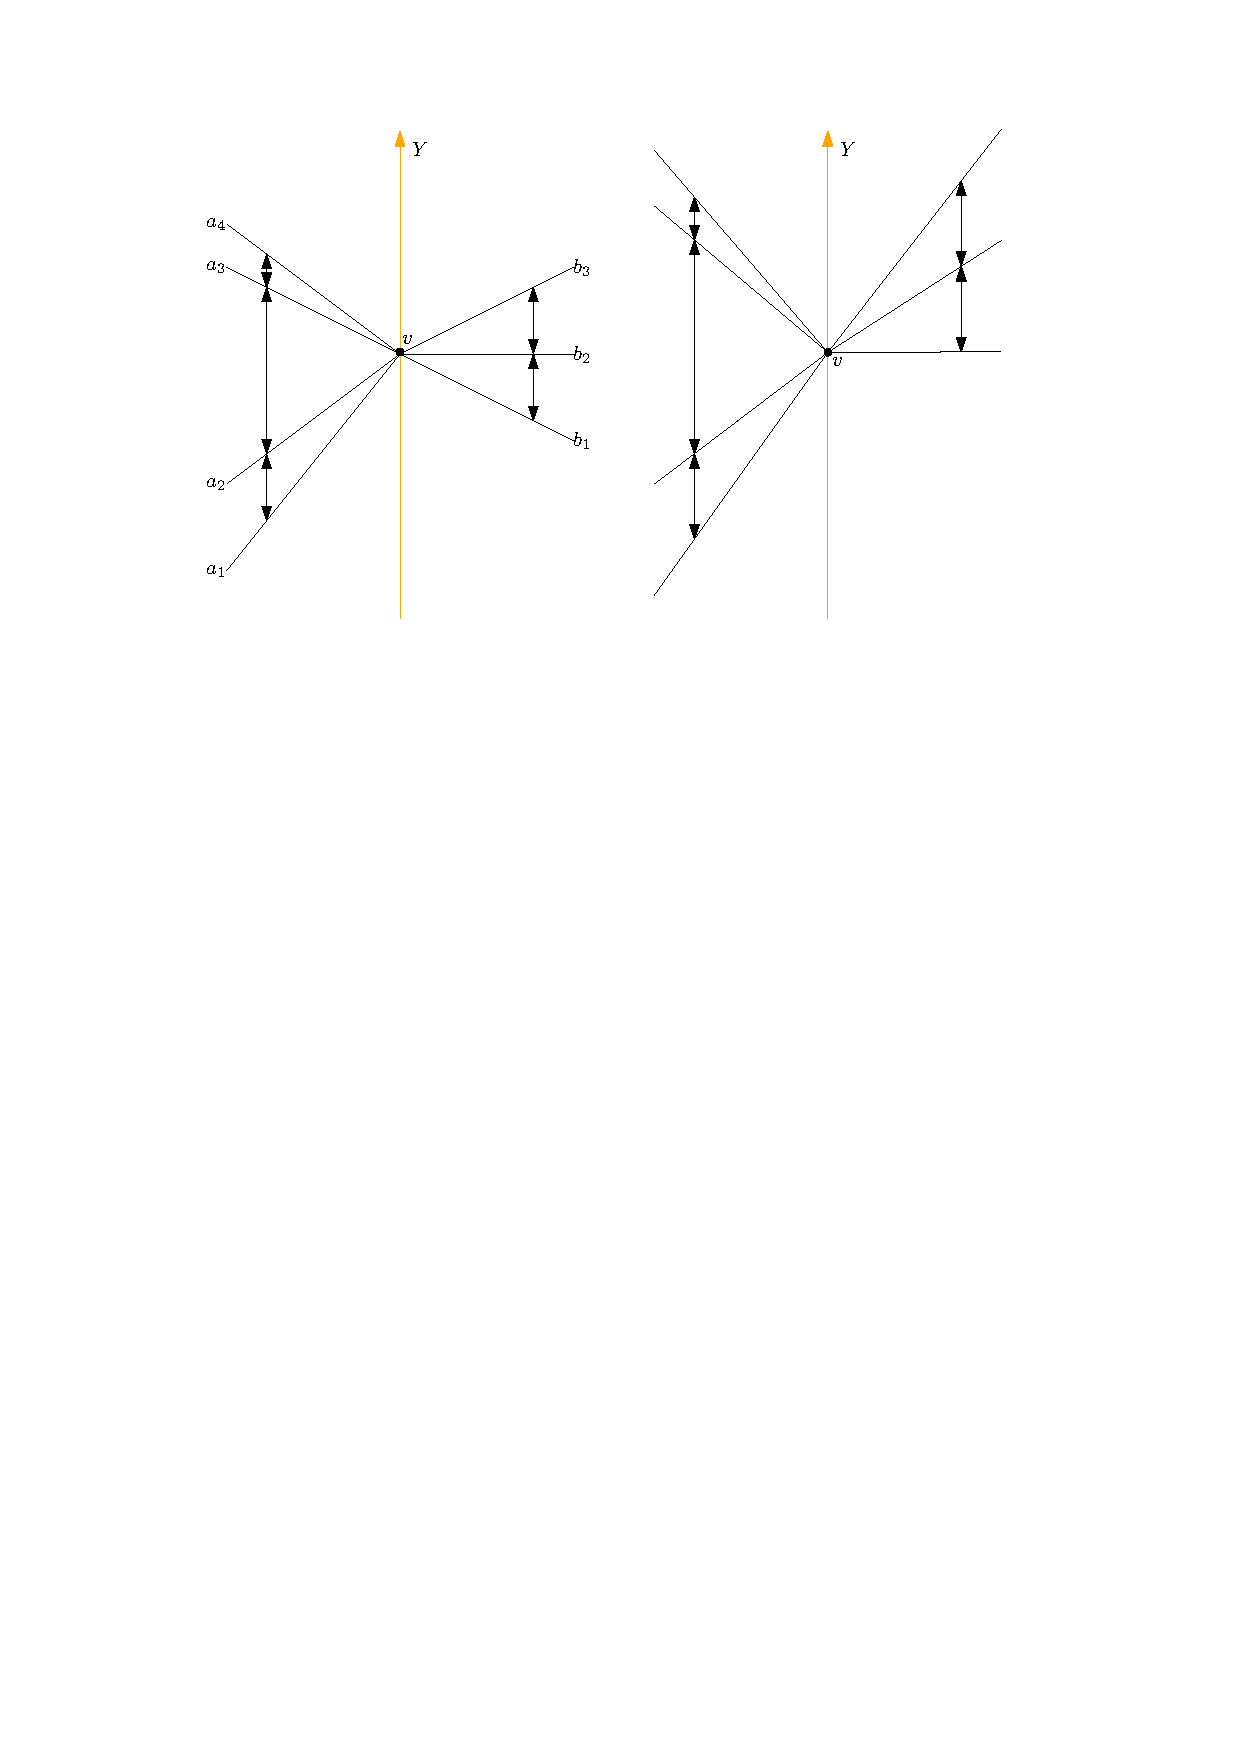
\includegraphics{figs/proportional}}
     \caption{The degrees of freedom provided by the proportionality constraints}
     \figlabel{proportional}
  \end{figure}
The total number of equations
\thetag{\ref{eq:slope0}--\ref{eq:proportion2}} turns out to be $m-4$.
This can be seen as follows: Let $n=|V|$ and let $n_0$ be the number
of vertices on $C$. Assume that $G$ has $f_3$ triangular and $f_4$
quadrangular faces.

Two triangles for every vertex on $C$ (Property X above):
\begin{equation}
  \label{eq:f3}
  f_3 = 2n_0
\end{equation}
Euler's formula:
\begin{equation}
  \label{eq:Euler}
  n + f_3+f_4 = m+2
\end{equation}
Double-counting of edge-face incidences leads to the relation
\begin{equation}
  \label{eq:edge-face}
  3f_3+4f_4=2m.
\end{equation}
We have $d_v-3$ for each of the $n_0$ vertices $v$ on $C$, if it has
degree $d_v$. For each of the 
 $n-n_0$ vertices $v$ not on $C$, 
we have $d_v-2$ equations.
  The total number of equations is therefore
  \begin{align*}
 % \label{eq:number-equations2}
G &= 
\sum_{v\in C}^n(d_v-3)+
\sum_{v\notin C}^n(d_v-2)
=
\sum_{v\in V}^n(d_v-2)-n_0
=
2m-2n-n_0.
  \end{align*}
Using \thetag{\ref{eq:f3}--\ref{eq:edge-face}}, this can be
simplified to
\begin{align*}
G&=
2m-2n-n_0\\
&= 2m -2n -2f_3-2f_4 +2f_3+2f_4-n_0\\
&= 2m -2(n +f_3+f_4) +\tfrac12(4f_3+4f_4-f_3)\\
&= 2m -2(m+2) +m = m-4.
\end{align*}

To achieve the desired number of $m$ equations, we have to add four
more equations.
If the outer face is a quadrilateral, we set the slopes of its
 4 edges
to fixed values.
If the outer face is a triangle $\alpha\beta\gamma$, with $\gamma$ on
$C$, we set the slopes of the 3 boundary edges
to fixed values. In addition, we pick another (non-boundary) edge
incident to $\gamma$ and set its slope to a fixed value.
(Together with the proportionality constraints, this effectively pins
all slopes
incident to $\gamma$ to a fixed value.)

We call these four additional equations the \emph{boundary equations}.

Altogether, we have now a system of $m$ linear equations
in the $m$ unknowns $s=(s_1,\ldots,s_m)$, which we can write
compactly as
 $A\cdot s = b$, with a square matrix $A$ whose entries come from
 \thetag{\ref{eq:slope0}--\ref{eq:proportion2}}.
%are the variables we wish to solve for, and $b$ is a column $m$-vector
%whose entries also come from \eqref{slope}.  
Only four entries of
the right-hand side vector
 $b$
are non-zero, due to the four boundary equations.
We will show that $A\cdot s=b$ has a unique
solution and that this solution gives a \Fary\ embedding of $Q$.

\subsubsection{Ordering constraints}

Define a relation $\prec$ on $\{1,\ldots,m\}$ where $i \prec j$
if
\begin{enumerate}
  \item $i < j$ and $e_i$ and $e_j$ are incident to a common vertex
  $v\in C^-$; or
  \item $i > j$ and $e_i$ and $e_j$ are incident to a common vertex $v\in C^+$.
\end{enumerate}
We say that a vector $s=(s_1,\ldots,s_m)$ \emph{satisfies the ordering constraints} if $s_i <
s_j$ for every pair $i,j\in\{1,\ldots,m\}$ such that $i\prec j$.  

This definition captures the condition that vertices inside of $C$
should be drawn to the left of the y-axis and those outside of $C$
should be drawn to the right of the y-axis.  It is straightforward
to verify that $\prec$ is actually a acyclic: We know that a
non-crossing drawing
$\bar D$ with the vertices on the correct side exists, and the slopes
$s_i'$ of that drawing must satisfy the ordering constraints.
%  Indeed, $i_1\prec
% \cdots \prec i_r$ implies that, for each $j\in\{3,\ldots,r\}$, $y_{i_j}\in
% (\min\{y_{i_{j-1}},y_{i_{j-2}}\}, \max\{y_{i_{j-1}},y_{i_{j-2}}\})$. Thus,
% a chain in $\prec$ corresponds to a sequence of strictly nested intervals.

\begin{lem}\lemlabel{order-gives-embedding}
   Any solution $s$ to $A\cdot s=b$ that satisfies
 the ordering constraints % $\prec$
 yields a
   \Fary\ embedding of $Q$.
\end{lem}

\begin{proof}
   If $G$ is a plane embedding of a 2-connected graph, then a
   straight-line embedding $G'$ of $G$ is a \Fary\ embedding provided
   that two conditions are met:
(i) For every vertex~$v$, the cyclic order of the
   edges around $v$ in $G'$ is the same as in $G$; and
(ii) every face of $G$ is embedded without crossings in $G'$
(Devillers, Liotta, Preparata, and Tamassia \cite[Lemma~16]{devillers.liotta.ea:checking}).

In our case, $G=Q$ and $G'=Q'$ is a straight-line embedding $Q'$ of
$Q$ given by a solution to $A\cdot s = b$.  For each vertex $v$ that
does not lie on $C$, the incident slopes satisfy the ordering constraints
by assumption, and hence the order of incident edges in $G'$ and $G$
agrees.

Let us consider a vertex $v$ on $C$, with
incident edges $a_1,\ldots,a_k$ 
on the left and $b_1,\ldots,b_l$ on the
right.
If $v$ is a boundary node, all slopes are fixed, and the cyclic order
is therefore correct.
Let us consider an interior vertex~$v$.
%
 As discussed above, the proportionality constraints ensure that
the cyclic order is either correct, or it is completely reversed on both
sides.
Let us assume for contradiction that the latter case happens:
\begin{equation}
  \label{eq:not-ordered}
s_{b_1}\ge s_{b_l}
\text{ and }
s_{a_k}\ge s_{a_1}
\end{equation}
Let $e$ be the third edge of the triangle with edges $a_1$ and $b_1$,
and let 
 $f$ be the third edge of the triangle with edges $a_k$ and $b_l$.
Then the ordering constraint for the endpoints of $e$ imply
\begin{math}
  s_{b_1}<s_e<s_{a_1}
\end{math},
and the ordering constraint for the endpoints of $f$ imply
\begin{math}
  s_{a_k}<s_f<s_{b_l}
\end{math}.
Together with \eqref{not-ordered}, this leads to a contradiction.

   For every quadrilateral face in $Q'$, the vertices don't lie on
   $C$, and the ordering constraints on the vertices
   ensure that the embedding is non-crossing. Therefore, by the result
   cited above, $Q'$ is a \Fary\ embedding. % of~$Q$.
\end{proof}


\subsubsection{Strong Ordering Constraints}
SAME AS SECTION \ref{strong}

\end{proof}

... UNTIL HERE CAN BE UNCHANGED.

 It remains to rule out the possibility that
 $A_{t^*}\cdot s=b_{t^*}$ has no solutions because
   $\lim_{t\uparrow t^*} s(t)$ does not exist.  Define the set $H=\{e_i\in
   \{e_1,\ldots,e_m\}:\text{$\lim_{t\uparrow t^*} s_i(t)$ exists}\}$.
(The set $H$ corresponds to edges of $Q$
   with
   bounded slope; the remaining edges have divergent slopes; they become vertical as $t\uparrow t^*$.)
The set   $H$ has the following
   properties:
GIVE THESE PROPERTIES A NAME OR PUT THEM IN A LEMMA, SO WE CAN REFER
TO THEM.
   \begin{enumerate}
    \item $H$ contains the edges
      on the outer face.
    \item
If a vertex $v$ that does not lie on $C$ has two incident edges in
$H$,
then all its incident edges belong to $H$.
    \item
If a vertex $v$ that lies on $C$ has two incident edges in
$H$ on the same side of $C$,
then all its incident edges belong to $H$.
    \item If $i \prec j \prec k$ and $e_i,e_k\in H$, 
      then $e_j\in H$.
   \end{enumerate}
Let us see why properties 2 and 3 are true.
If $v$ does not lie on $C$ and two incident edges have a convergent
slope, this means that the location of $v$ is fixed in the limit.
By the concurrency equations, the slopes of the remaining incident
edges are also determined, by the requirement that the edges go through
the limit location of $v$.

If $v$ lies on $C$, the argument is more elaborate. If $v$ lies on
$C$, then all incident edges have fixed slopes and are therefore in
$H$.
Let uus consider the case that $v$ is an interior vertex.
As above, defince the incident edges $a_i$ and $b_j$.
Let $e$ be the third edge of the triangle with edges $a_1$ and $b_1$,
and let 
 $f$ be the third edge of the triangle with edges $a_k$ and $b_l$.
Assume without loss of generality that two of the edges $a_i$ on the
left belong to $H$. Then, by the proportionality constraints, all
left edges $a_i$ belong to $H$, and moreover, the range $b_l-b_1$ of
the right incident edges converges to a bounded limit.
It follows that either all the right edges $b_j$ converge, 
or they all diverge to $+\infty$,
or they all diverge to $-\infty$,
Then the ordering constraint for the endpoints of $e$ imply
\begin{math}
  s_{b_1}<s_e<s_{a_1}
\end{math}.
THERE IS SOME REPETITIVENESS HERE.
This is inconstent with $\lim s_{b_1}=+\infty$.
The ordering constraint for the endpoints of $f$ imply
\begin{math}
  s_{a_k}<s_f<s_{b_l}
\end{math}.
This is inconstent with $\lim s_{b_l}=-\infty$.
Thus, the only possibility is that all incident slopes converge.

We have now established that the set $H$ has
 the above four properties.
   \lemref{partition-extended} below shows that such a set
   $H$ contains all edges. All slopes converge, and this 
   completes the proof.
\qed%\end{proof}

%Condition 1 in the following lemma is more general that what we need,
%because it allows us to proceed by induction.

\begin{lem}\lemlabel{partition-extended}
(TAKES THE ROLE OF PREVIOUS LEMMA 5, now \lemref{partition}.)
  Let $Q$ be a graph (a ``near-A-graph''?) in which every edge is intersected
  by $C$, and each inner face is a triangle or quadrilateral, and each
  vertex on $C$ has neighbors on the left and on the right.  Let $H$
  be a subset of $E(Q)$ such that
   \begin{compactenum}
    \item If $v$ is a vertex on the outer face 
      of $Q$, then all incident edges belong to $H$;
    \item
If a vertex $v$ that does not lie on $C$ has two incident edges in
$H$,
then all its incident edges belong to $H$.
    \item
If a vertex $v$ that lies on $C$ has two incident edges in
$H$ on the same side of $C$,
then all its incident edges belong to $H$.
    \item if $i \prec j \prec k$ and $i,k\in H$, 
      then $j\in H$.
   \end{compactenum}
   Then $H=E(Q)$.
\end{lem}

This lemma applies to a more general class of graphs than we
need,
because if imposes no constraints on the outer face.
This will allow us to prove it by induction.

 Assumption 1 is nominally stronger than what we have proved above.
Let us see why it is true: Initially, a boundary vertex
 can
lie on $C$ as a vertex of a triangle, then all incident edges belong to $H$ because their slopes
are fixed,
or it
 can
lie on $C$ as a reflex vertex of a quadrilateral, then there are two
$H$-edges on the same side,
or it can
lie away from $C$, then again there are two
incident $H$-edges.
In all cases, we can conclude that all incident edges belong to $H$.


\begin{proof}
The proof is by induction
   on the lexicographically ordered pair $(f(Q),|E(Q)|)$, where $f(Q)$
is the number of inner faces of $Q$. 
More specifically, %In other words
%We prove the claim by dismantling $Q$
we will dismantle $Q$
 from outside while maintaining
 Conditions 1--4:
\begin{itemize}
\item If $Q$ is not 2-connected but has more than one edge, we cut it
  into pieces with fewer edges.
\item If $Q$ is 2-connected, we will modify it and reduce it to a
  graph
with fewer interior faces,
keeping the number of edges fixed.
\end{itemize}
Eventually, we reduce to a graph with a single edge, and here the
claim is trivial because the edge belongs to the boundary.

   We refer to the edges of $H$ simply as \emph{$H$-edges}.
% (horizontal edge) if it is
%   in $B$ and a \emph{v-edge} (vertical edge) otherwise.  Thus, we wish
%   to show that all edges of $Q$ are h-edges. 
The edges on the outer
   face are called boundary edges.

If $Q$ is not connected then we can apply induction to each component
   of $Q$ separately. If $Q$ has a cut vertex $v$, whose removal
   separates $Q$ into components $A_1,\ldots,A_r$ then, for each
   $i\in\{1,\ldots,r\}$, we can apply induction to the subgraph of $Q$
   induced by $V(A_i)\cup\{v\}$.  
In these reductions, no new boundary edges appear that were not
previously boundary edges, because each inner face is
a quadrangle or a triangle: $Q$ cannot contain a nested (2-connected) component
inside another face.
Some adjacent edges in $Q$ might no longer be adjacent
after we cut $Q$ into pieces. This can make Conditions 2 and~3 only weaker
when applied to the pieces. Thus, induction is justified.

----  FROM HERE ON ONLY SKETCHY -----

IN PARTICULAR: NEED TO RE-ESTABLISH PROPERTY 1.

We are left with the case that $Q$ is a 2-connected \emph{near-A-graph}(?) whose outer face 
   is a simple cycle $F$.

Case 1. $F$ contains a vertex $v$ on $C$.
Then we identify an interior triangle incident to $v$ and open it up,
merging it into the outer face, see \figref{lemma-y-3}.

  \begin{figure}
     \centering{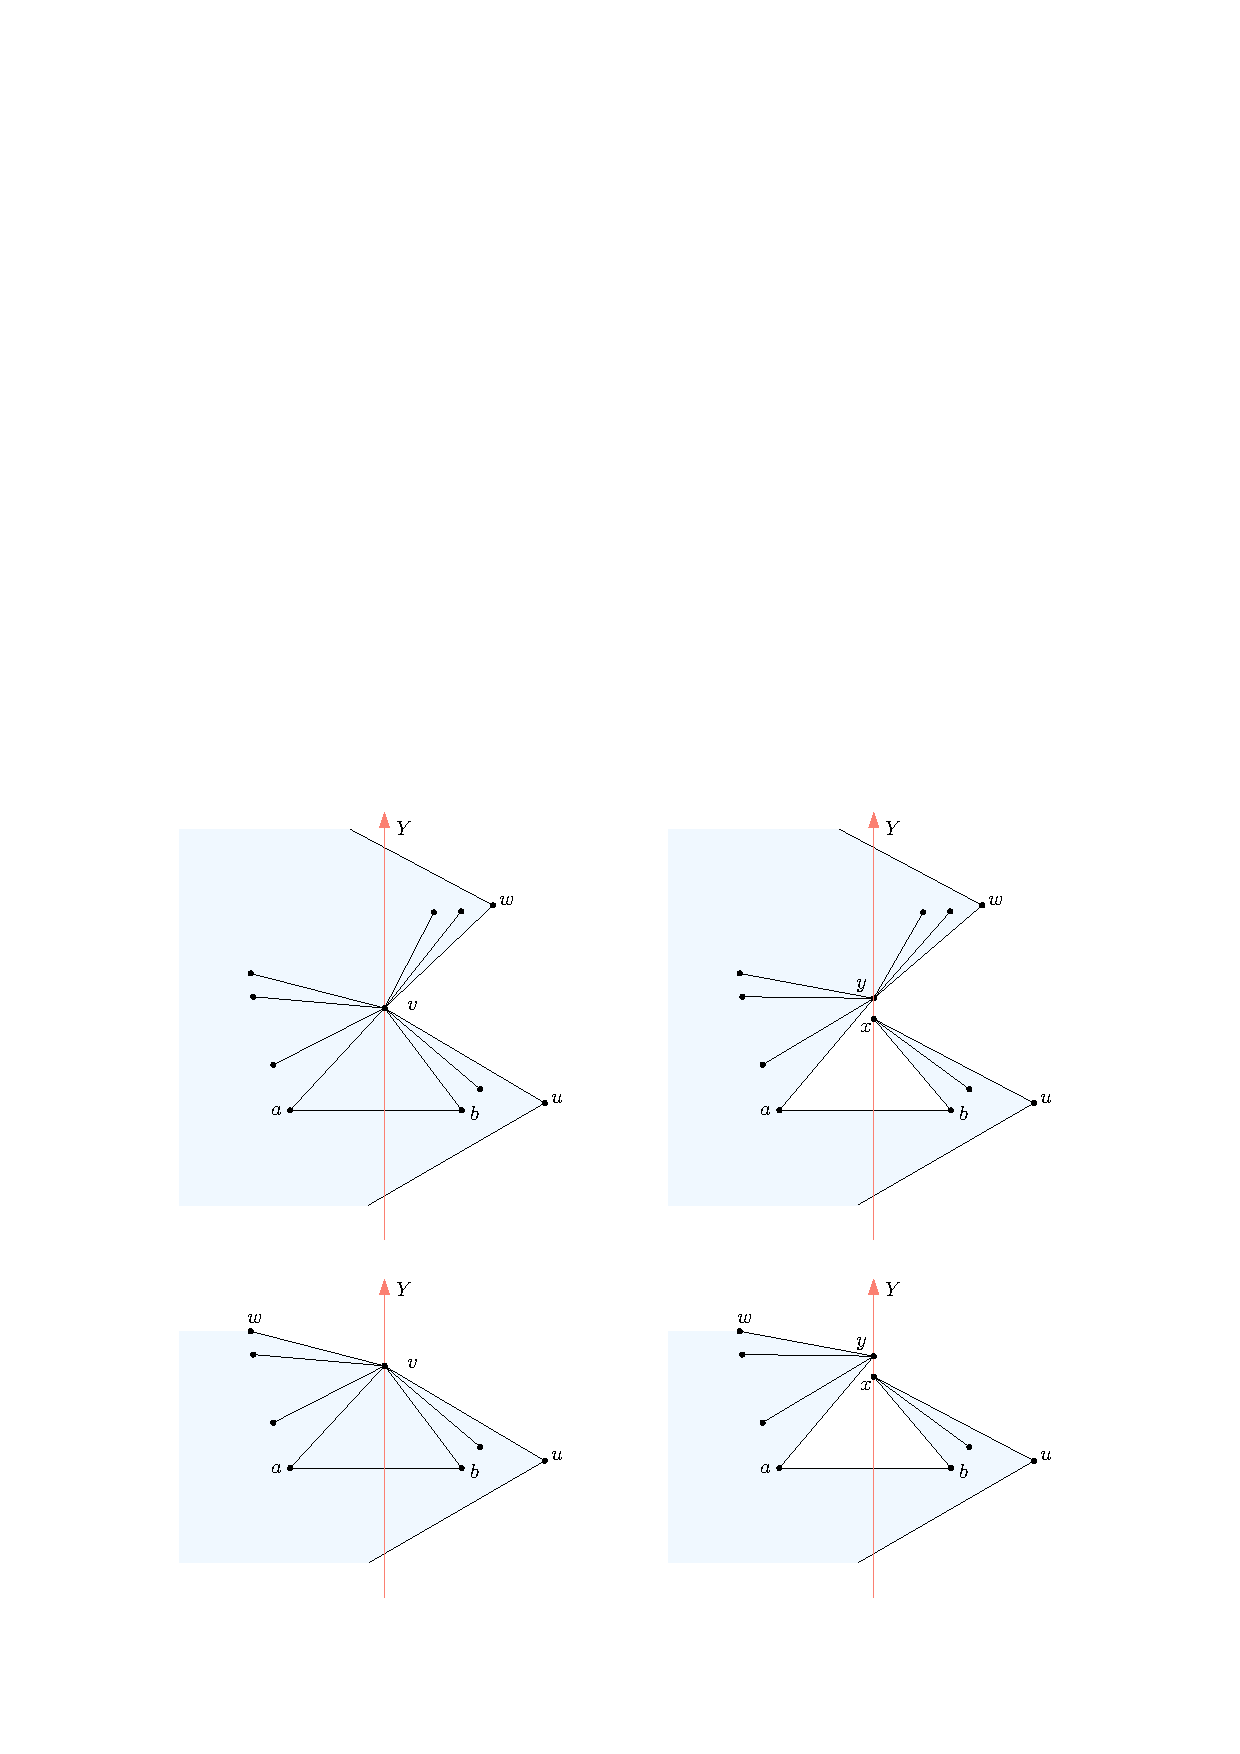
\includegraphics{figs/open-a-triangle}}
     \caption{Proof of \lemref{partition-extended} for a vertex
       $v$ on $C$. Integrating a triangle in the outer face.}
     \figlabel{lemma-y-3}
  \end{figure}
   
Case 2. $F$ contains no vertex on $C$.
%  The outer face of $Q$ is a  simple cycle,
$F$ contains at least four vertices, and $C$ intersects
   every edge of $F$.  Therefore,  
   $F$
    must contain three consecutive vertices
   $u,v,w$ such that $C$ exits an inner face through $uv$ and enters
   an inner face through $vw$, see \figref{lemma-y-4}.
  This implies that $v$ is a reflex vertex
   of some bounded face $q=vabc$ of $Q$.  Indeed, $vc$ is the first edge
   incident to $v$ crossed by $C$ and $va$ is the last edge incident to
   $v$ crossed by $C$.

  \begin{figure}
     \centering{\includegraphics{figs/lemma-y}}
     \caption{Proof of \lemref{partition-extended} for a reflex
       vertex $v$. Integrating a quadrilateral in the outer face.}
     \figlabel{lemma-y-4}
  \end{figure}
   

   We construct a new graph $Q'$ by splitting $u$ into two vertices $x$
   and $y$.  We make the vertex $x$ adjacent to $u$ and every neighbour
   $z$ of $v$ such $C$ intersects $vz$ before it intersects $vu$.  We make
   $y$ adjacent to all of $v$'s neighbours that are not adjacent to $x$.
   In $Q'$, $q$ is part of the outer face, so $Q'$ has one less inner
   face than $Q$, while having the same number of edges.

We have to show that the edges of the quadrilateral 
$q=vabc$,
which become boundary edges of $Q'$, are $H$-edges.
The reflex vertex $v$ is incident to two $H$-edges, namely those of
$F$, and therefore, by Condition 2, $va,vc\in H$.
By looking at the vertices of $q$, we get
$vc \prec bc\prec ba\prec va$ or 
$va \prec ba\prec bc\prec vc$,
 depending on whether $v\in C^-$ or
$v\in C^+$. 
Thus, by Condition~3, $bc$ and $ba$ are also $H$-edges.

Every edge of $Q'$ inherits its classification as an $H$-edge from
its corresponding edge in $Q$.
   In $Q'$ some of the $\prec$ relations involving edges incident
   to $v$ are missing, but no new ones are introduced, so $Q'$ still
   satisifies Condition~3.
The same argument applies to
Condition~2. Some adjacent edges in $Q$ might no longer be adjacent
in $Q'$, but this makes Condition 2 only weaker. (REPETITION!)


   By Conditions~1 and 2, all edges incident to $v$ are $H$-edges and $v$
   is a reflex vertex of $q$. Therefore all edges of $q$ are $H$-edges.
We have justified the induction step for the case when $Q$ is
2-connected, and
   the proof is complete.
\end{proof}


END OF NEW STUFF
\hrule


%%% Local Variables:
%%% mode: latex
%%% TeX-master: "freecoll"
%%% End:
